\chapter{Binary Shift Keying}

Orthonormal carrier signals in each modulation scheme are: \\[10pt]

\newcommand{\se}{\sqrt{\dfrac{2E_b}{T_b}}}

\begin{center}
	\begin{tabular}{|c|c|}
\hline
BASK & \makecell{$\begin{aligned}
s_1(t) &= \se \cos(2\pi f_c t) \\[10pt]
s_2(t) &= 0
\end{aligned}$} \\ \hline
BPSK & \makecell{$\begin{aligned}
	s_1(t) &= \se \cos(2\pi f_c t) \\[10pt]
	s_2(t) &= \se \cos(2\pi f_c t + \pi)
\end{aligned}$} \\ \hline
BFSK & \makecell{$\begin{aligned}
	s_1(t) &= \se \cos(2\pi f_{c1} t) \\[10pt]
	s_2(t) &= \se \cos(2\pi f_{c2} t)
\end{aligned}$} \\ \hline
\end{tabular}
\end{center}
Transmitted wave is given by

\begin{equation*}
s(t) = \begin{cases}
		s_1(t)  &  \text{if bit = 1} \\
		s_2(t)  &  \text{if bit = 0}
	\end{cases}
\end{equation*}
For demodulation, refer: \nameref{mary}

Throughout the entire program (and in other programs like line codes, etc), I've used \texttt{kron} function. more on that function below:
\section*{\texttt{kron} function \label{kronfx}}
\texttt{kron} is used to implement \href{https://en.wikipedia.org/wiki/Kronecker_product}{Kronecker product} which is here used to create copies of a carrier signal based on the message signal.
Kronecker product of two matricies $A = \begin{bmatrix}1 & 2 & 3\end{bmatrix}$ and $B = \begin{bmatrix}1 & 1 & 0 & 0\end{bmatrix}$ is:

$$\begin{aligned}
	A \otimes B &= \begin{bmatrix}1 & 2 & 3\end{bmatrix} \otimes \begin{bmatrix}1 & 1 & 0 & 0\end{bmatrix} \\
&= \begin{bmatrix}
1 \begin{bmatrix}1 & 1 & 0 & 0\end{bmatrix} & 
2 \begin{bmatrix}1 & 1 & 0 & 0\end{bmatrix} & 
3 \begin{bmatrix}1 & 1 & 0 & 0\end{bmatrix}
\end{bmatrix} \\
&= \left[\begin{array}{cccccccccccc}
	1 & 1 & 0 & 0 & 2 & 2 & 0 & 0 & 3 & 3 & 0 & 0
\end{array}\right]
\end{aligned}
$$

From this you can see \texttt{kron} can produce any required copies of a carrier signal based on message bit stream:

\begin{figure}[!ht]
	\centering
	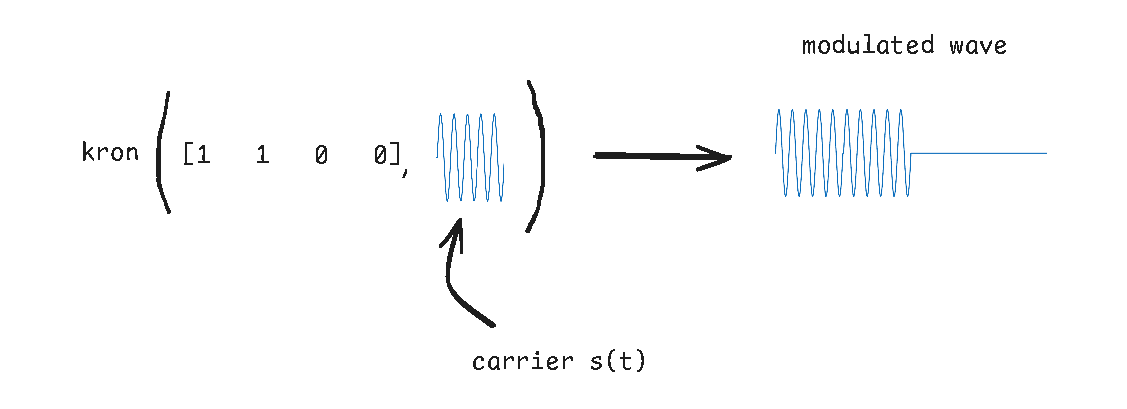
\includegraphics[width=\textwidth]{img/kron.pdf}
\end{figure}

This function is used extensively throughout the remaining MATLAB codes in this PDF.

\section*{Program}
\importMLCode{code/bsk.m}

\begin{figure}[!ht]
	\centering
	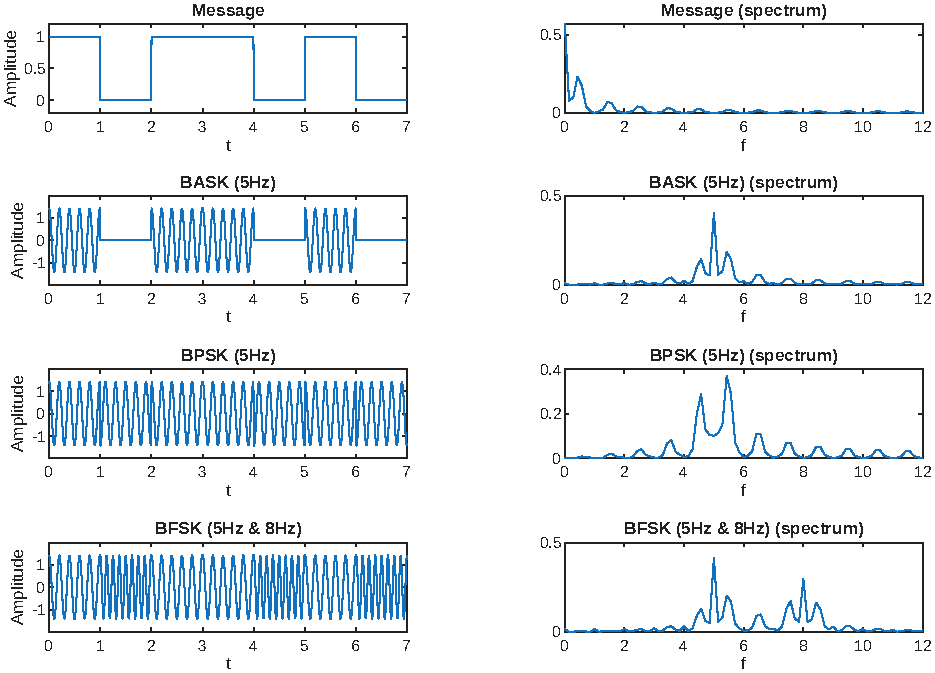
\includegraphics[width=\textwidth]{img/bsk.pdf}
\end{figure}


